\documentclass[12pt, twoside]{article}
\usepackage[francais]{babel}
\usepackage[T1]{fontenc}
\usepackage[latin1]{inputenc}
\usepackage[left=5mm, right=5mm, top=4mm, bottom=4mm]{geometry}
\usepackage{float}
\usepackage{graphicx}
\usepackage{array}
\usepackage{multirow}
\usepackage{amsmath,amssymb,mathrsfs}
\usepackage{soul}
\usepackage{textcomp}
\usepackage{eurosym}
 \usepackage{variations}
\usepackage{tabvar}


\pagestyle{empty}

\begin{document}


\begin{center}
\Large{\textbf{Devoir maison 7}}
\end{center}


\medskip


\textit{Devoir � rendre sur feuille grand format pour le \ul{jeudi 17 avril 2014}. Chaque r�ponse sera justifi�e.}

\medskip



\ul{Exercice 1}: \textit{(4 points)}



Le stade du Parc des Cygnes peut contenir 15 000 places. Il y a $x$ places en
virage, les autres en tribune. Les places en virage co�tent 10 \euro, les
places en tribune co�tent 13 \euro. Aujourd'hui, le stade est plein.

\begin{enumerate}
  \item Que repr�sentent les trois expressions suivantes:
 \qquad  $10x$ \qquad \qquad  $15 000-x$ \qquad \qquad  $(15 000-x) \times
  13$
  
  \item Ecrire en fonction de $x$ le montant total de la recette (c'est-�-dire
  la somme d'argent gagn�e par la vente des billets.)
  \item Calculer cette recette si x=6500.
\end{enumerate}

\medskip




\ul{Exercice 2}: \textit{(4 points)}



R�duire les expressions suivantes:
\qquad A=(2x+7)+(3x-6)-(-5-x) \qquad \qquad B=-(5+4y)-(4-4y)+(-3+y)



\medskip


\ul{Exercice 3}: \textit{(3 points)}



\textit{ex 24 p 85 du manuel}

\medskip



\ul{Exercice 4}: (\textit{4 points})



On a relev� la nationalit� des vainqueurs de 97 tours de France de cyclisme
entre 1903 et 2010. Le tableau ci-dessous donne les nationalit�s des vainqueurs
et la fr�quence de victoires.

\begin{center}
\begin{tabular}{|c|c|c|c|c|c|}
\hline
Pays & France & Belgique & Espagne & Etats-Unis & Autres \\

\hline

Nombre de victoires & 36 & 18 & 13 & 10 & 20 \\

\hline

fr�quence en \% & \ldots \ldots & 18,6 & 13,4 & 10,3 & 20,6 \\

\hline
\end{tabular}
\end{center}


\begin{enumerate}
  \item Calculer la fr�quence en pourcentage de victoires fran�aises, arrondie
  � 0,1\% pr�s.
  \item On veut r�aliser un diagramme circulaire repr�sentant la r�partition
  des nationalit�s des vainqueurs.
  
  \begin{enumerate}
    \item Calculer les mesures d'angles repr�sentant les victoires de chaque
    pays, arrondie au degr� pr�s. On pourra faire un tableau de
    proportionnalit�.
    \item Construire ce diagramme circulaire.
  \end{enumerate}
  
\end{enumerate}


\medskip



\ul{Exercice 5}: (\textit{2 points})




Un serveur dans un bar  fait le bilan des pourboires qu'il a gagn�s chaque
jour. Calculer la moyenne journali�re de ses pourboires.


\begin{center}
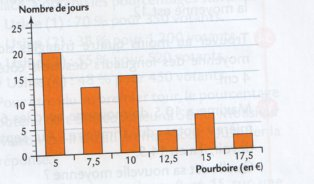
\includegraphics[width=9cm]{images/ex4.jpg}
\end{center}


\medskip



\ul{Exercice 6 }: (\textit{3 points})



Dans une salle de concert, le niveau sonore est affich� toutes les minutes.
Voici les relev�s (en d�cibels) au cours d'une demi-heure:

\begin{center}
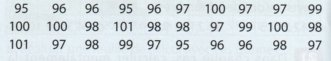
\includegraphics[width=7cm]{images/ex6.jpg}
\end{center}


\begin{enumerate}
  \item Pr�senter ces donn�es dans un tableau d'effectifs.
  \item Calculer le niveau sonore moyen.
\end{enumerate}

\end{document}


